
\chapter{DESIGN DETAILS AND IMPLEMENTATION}
\section{Compartment Description}

The computer nodes are grouped into two parts: \rom{1}. targeted nodes and \rom{2}. attacker nodes. In the proposed model, targeted population is subdivided into four compartments namely Susceptible, Infected, Quarantine and Recovered, while attacker population consists of into three compartments: Infected, Breaking-out and Recovered.
 Here, total computer nodes fall into seven classes, namely,
  \begin{enumerate}
    \item $S_1(t)$  susceptible nodes of targeted class,
    \item $I_1(t)$  infected nodes of targeted class;
    \item $I_2(t)$  infected nodes of attacker class;
    \item $Q_1(t)$  quarantined nodes of targeted class;
    \item $B_2(t)$  infected nodes of attacker class in breaking-out state of malicious code and
    \item $R_1(t)$  recovered nodes of targeted class
    \item $R_2(t)$  recovered nodes of attacker class
  \end{enumerate}
 The schematic flow of the model is shown in figure \ref{13-DR1}. Here some assumptions, i.e., the law of mass action and homogeneous spatial distribution in the mixing of hosts is taken into consideration, i.e., through out the total size of population, the density of the local population remains constant.
Targeted population:
\begin{equation} \tilde N_1(t) =\tilde S_1 (t)+\tilde I_1 (t)+\tilde Q_1 (t)+ \tilde R_1 (t), \end{equation} and attacker population:
\begin{equation}\tilde N_2(t) =\tilde I_2 (t) +\tilde B_2 (t) + \tilde R_2 (t) . \end{equation}
\par
The primary objective of this model is to analyze the effect of parameters used during transmission of information to control the transmission of malicious codes. Some researchers explored the impact of media awareness in biological disease spread using mathematical modeling with transmission coefficient function
\begin{equation} \beta (I) = \beta e^{-m I/N}, \end{equation} and noticed that many positive equilibria are possible when the effect of media is adequately
 sturdy among the population \cite{edtr10,edtr11,edtr12,edtr13}.
\par
Similarly, infection controlling factor on behalf of media coverage '$m$' is taken into consideration. The factor '$m$' depends on the types of files under review, defined firewall security rules in the firewall rule base and the reliability and efficiency of the
 firewall or any other media coverage factor. The objective of this thesis is to analyze various aspects of malicious code propagation within the computer network.

In the mathematical modeling of propagation of the malicious codes, the incidence function has a significant role. In various mathematical models, $\beta$ $SI$ is used as
 the bilinear incidence rate and $\beta$ $SI/N$ is used as the standard occurrence rate, where $\beta$ quantifies the effect of both the contact transmission rates
 and the propagation of the malicious object(code). However, the impact of any media coverage factor like firewall security to the spread and control of malicious code
 propagation is not considered in these occurrence function.
\par Initially, the expression for transmission rate \begin{equation*} \beta (I) = \beta e^{-m I}, \end{equation*} is used by the researchers but it has some faults.
So, firewall (media coverage factor) induced contact transmission rate as \begin{equation*} \beta (I) = \beta e^{-m I/N}, \end{equation*} is used in
the compartmental model which is more rational, because
\begin{equation*} \beta (I) = \beta e^{-m I/N}\rightarrow 0 \hspace{1 cm} \ \mbox{as} \ \hspace{1 cm} I \rightarrow \infty, \end{equation*}
independent of the nature of $m$. It is seen that the firewall security and vigilance are only the extrinsic deterministic transmission factor,
so it is logical to consider that the rate of transmission cannot be decreased below a threshold level simply through the firewall security alert.
 Besides further for a fixed value of $m$, the minimum rate of transmission varies with size of the population, which is impractical.
\begin{equation*}min\{\beta e^{-m I/N}= \beta e^{-m} \} \end{equation*}
 which remains unchanged with the population size\cite{edtr15,edtr19}.


 \clearpage

\section{Mathematical Model and Schematic Flow Diagram}
\begin{figure}[h]
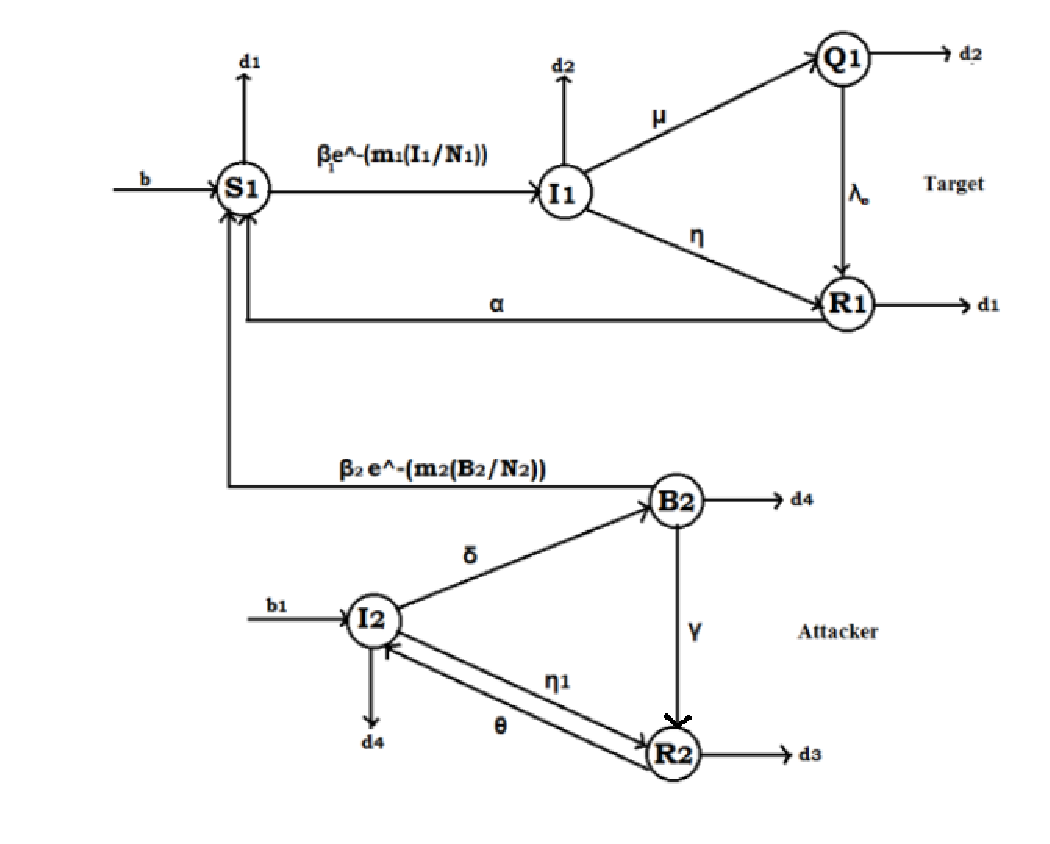
\includegraphics[width=5.7in]{13-DR1}

\caption{Schematic Flow Diagram of the model}
\label{13-DR1}
\end{figure}

Considering the transmission rates shown in the figure \ref{13-DR1}, the following set of ordinary differential equations represents the propagation of malicious codes :\\
{\bf For targeted nodes:}
\begin{eqnarray}
% \nonumber % Remove numbering (before each equation)
  \frac{d \tilde S_1}{d \tilde t}  &=&  b-d_1 \tilde S_1+ \tilde \alpha \tilde R_1 - \tilde \beta_1 e^{-m_1 \left(\frac{ \tilde I_1}{ \tilde N_1}\right)}\left(\frac{ \tilde I_1}{ \tilde N_1}\right) \tilde S_1- \tilde \beta_2 e^{-m_2 \left(\frac{ \tilde B_2}{ \tilde N_2}\right)} \left(\frac{ \tilde B_2}{ \tilde N_2}\right) \tilde S_1, \\
   \frac{d \tilde I_1}{d \tilde t} &=& \tilde \beta_1 e^{-m_1 \left(\frac{\tilde I_1}{\tilde N_1}\right)}\left(\frac{\tilde I_1}{\tilde N_1}\right) \tilde S_1+\tilde \beta_2 e^{-m_2 \left(\frac{\tilde B_2}{\tilde N_2}\right)} \left(\frac{\tilde B_2}{\tilde N_2}\right)\tilde S_1 - (\tilde d_2+ \tilde\eta +\tilde \mu)\tilde I_1, \\
  \frac{d \tilde Q_1}{d \tilde t} &=& \tilde \mu \tilde I_1 -\tilde d_2 \tilde Q_1 - \tilde \lambda_0 \tilde Q_1, \\
 \frac{d \tilde R_1}{d \tilde t} &=&  \tilde\lambda_0 \tilde Q_1-\tilde \alpha \tilde R_1-d_1 \tilde R_1+ \tilde\eta \tilde I_1 .
\end{eqnarray}

{\bf For attacker nodes:}
\begin{eqnarray}
% \nonumber % Remove numbering (before each equation)
 \frac{d \tilde I_2}{d \tilde t} &=& b_1- \tilde d_4 \tilde I_2-\tilde \delta \tilde I_2 +\tilde \theta \tilde R_2 -\tilde\eta_1 \tilde I_2, \\
 \frac{d \tilde B_2}{d \tilde t} &=& \tilde\delta\tilde I_2 -\tilde d_4 \tilde B_2 -\tilde\gamma\tilde B_2 ,\\
\frac{d \tilde R_2}{d \tilde t} &=& \tilde\gamma \tilde B_2 - d_3 \tilde R_2 - \tilde \theta\tilde R_2+\tilde \eta_1\tilde I_2 .
\end{eqnarray}
\par where every system parameter is positive and illustrated in table \ref{table:param1a}.
\begin{table}
\begin{tabular}{|p{3 cm}|p{11 cm}|}
\hline
\bf Parameters & \bf Description \\
\hline
b, $b_1$ & Recruitment rates of target and attacker classes\\
\hline
$d_1$, $d_3$ & Natural death rate of targeted and attacker population node\\
\hline
$\beta_1$ & Contact rate from susceptible class to infected class\\
\hline 
$\beta_2$ & Contact rate from breaking-out to susceptible class\\
\hline
$\gamma$ &Rate of recovery of computers with malicious codes in breaking-out state\\
\hline
$\eta$, $\eta_1$ &Rate of recovery of computers with malicious codes in infected state\\
\hline
$d_2$ &Death rate in infected target classes(death due to infection and natural death)\\
\hline
$\lambda_0$ &Rate of recovery of computers with malicious codes in quarantine state\\
\hline
$\delta$ &Rate of change of malicious nodes from infected to breaking-out state\\
\hline
$\theta$ &Rate of change of recovered nodes into infected nodes(immunity loss)\\
\hline
$d_4$ &Death rate in infected attacker classes(death due to infection and natural death)\\
\hline
$\alpha$ &Rate of change of recovered nodes into susceptible nodes\\
\hline
$m_1$, $m_2$ &Infection controlling coefficients\\
\hline
$\mu$ &Rate of change of malicious nodes from infected to quarantine state\\
\hline
\end{tabular}
\caption {Description of Parameters}
\label{table:param1a}
\end{table}
\clearpage
\section{Non-dimensionalisation}
Due to complicated nature of the equations (2.4)-(2.10), these equations are non-dimensionalized for the above system using:

\begin{equation*}
S_1=\frac{ \tilde S_1}{ \tilde N_1}, \hspace{0.5 cm} I_1=\frac{ \tilde I_1}{ \tilde N_1}, \hspace{0.5 cm} Q_1=\frac{ \tilde Q_1}{ \tilde N_1}, \hspace{0.5 cm}
R_1=\frac{ \tilde R_1}{\tilde N_1},\end{equation*}
\begin{equation*}I_2=\frac{ \tilde I_2}{\tilde N_2},  \hspace{0.5 cm} B_2=\frac{\tilde B_2}{\tilde N_2},  \hspace{0.5 cm} R_2=\frac{\tilde R_2}{\tilde N_2}, \hspace{0.5 cm} t=\tilde d_1 \tilde t,\end{equation*}
\begin{equation} N_1=\frac{\tilde N_1}{ \tilde N_1\textsuperscript{0}},  \hspace{0.5 cm} N_2=\frac{\tilde N_2}{ \tilde N_2\textsuperscript{0}},  \hspace{0.5 cm} \tilde N_1\textsuperscript{0}=\frac{b}{\tilde d_1},  \hspace{0.5 cm} \tilde N_2\textsuperscript{0}=\frac{b_1}{\tilde d_3}.
\end{equation}
The equivalent non-dimensional system is given by:\\
{\bf For targeted nodes:}
\begin{eqnarray}
\frac{d S_1}{dt} &=& \frac{( 1- S_1)}{N_1}+ \alpha R_1 - \beta_1 e^{-m_1 I_1} I_1 S_1- \beta_2 e^{-m_2 B_2} B_2 S_1-S_1+S_1^2 \nonumber \\
&+& d_2 I_1 S_1+d_2 Q_1 S_1+R_1 S_1,
\end{eqnarray}
\begin{eqnarray}
\frac{d I_1}{dt}&=& \beta_1 e^{-m_1 I_1} I_1 S_1 +\beta_2 e^{-m_2 B_2} B_2 S_1 - ( d_2+ \eta + \mu) I_1- \frac{ I_1}{N_1}+d_2 I_1^2 \nonumber\\
&+& I_1 S_1+d_2 Q_1 I_1+I_1 R_1,
\end{eqnarray}
\begin{equation}
\frac{d Q_1}{dt}= \mu I_1 - d_2 Q_1 - \lambda_0 Q_1- \frac{ Q_1}{N_1}+d_2 Q_1^2+d_2 I_1 Q_1+ Q_1 S_1+Q_1 R_1,
\end{equation}
\begin{equation}
\frac{d R_1}{dt}=\lambda_0 Q_1- \alpha R_1- R_1+ \eta I_1- \frac{ R_1}{N_1}+R_1^2+d_2 I_1 R_1+d_2 Q_1 R_1+R_1 S_1 .
\end{equation}

{\bf For attacker nodes:}
\begin{eqnarray}
% \nonumber % Remove numbering (before each equation)
  \frac{d I_2}{dt }&=&  \frac{( 1- I_2)}{N_2}- d_4 I_2-\delta I_2 + \theta R_2 -\eta_1 I_2+ d_4 I_2^2+d_4 I_2 B_2+ I_2 R_2, \\
 \frac{d B_2}{d t}&=& \delta I_2 - d_4 B_2 -\gamma B_2- \frac{ B_2}{N_2}+d_4 B_2^2+d_4 I_2 B_2+ B_2 R_2 , \\
   \frac{d R_2}{d t} &=& \gamma B_2 - R_2 - \theta R_2+ \eta_1 I_2- \frac{ R_2}{N_2}+R_2^2+d_4 I_2 R_2+d_4 B_2 R_2 .
\end{eqnarray}

Where population parameters of both classes are dimensionalised by $d_1$ and $d_3$ respectively.
\clearpage
\section{Boundedness of the System}
For the verification of boundedness of the defined system, the systems is classified into two parts, i.e., targeted and the Attacker Population. For targeted population, the equations are:

\begin{equation*} \tilde N_1(t) =\tilde S_1 (t)+\tilde I_1 (t)+\tilde Q_1 (t)+ \tilde R_1 (t),\end{equation*}
then,
\begin{equation*}\frac{d \tilde N_1}{d \tilde t} = \frac{d \tilde S_1}{d \tilde t}+\frac{d \tilde I_1}{d \tilde t}+
\frac{d \tilde Q_1}{d \tilde t}+\frac{d\tilde R_1}{d \tilde t},\end{equation*}
\begin{equation} \frac{d \tilde N_1}{d \tilde t}=b-\tilde d_1 \tilde S_1-\tilde d_2 \tilde I_1-\tilde d_2 \tilde Q_1-\tilde d_1 \tilde R_1\end{equation}
Again, let
\begin{equation*} d = min\{\tilde d_1,\tilde d_2\},\end{equation*}
then,
\begin{equation*}\frac{d \tilde N_1}{dt} \leq b - d[ \tilde S_1 + \tilde I_1 + \tilde Q_1 + \tilde R_1] = b - d \tilde N_1. \end{equation*}
If \begin{equation*} \tilde N_1(t) > (b/d), \ \mbox{then} \ \frac{d \tilde N_1}{d t} < 0,\end{equation*} implying \begin{equation*}lim_{t \rightarrow \infty} \tilde N_1(t)\leq b/d .\end{equation*}
It can be seen after a moment of observation, that, simply connected compressed set
\begin{equation}\Omega_k = \{( \tilde S_1, \tilde I_1, \tilde Q_1, \tilde R_1) \in R_+ \textsuperscript{4} : \tilde S_1+ \tilde I_1 + \tilde Q_1 + \tilde R_1 \leq b/d \},\end{equation}
is positively invariant for the model. Hence, the suggested system is well mannered.
Similarly, boundedness of the Attacker nodes can also be defined.
\begin{equation*} \tilde N_2(t) =\tilde I_2 (t)+\tilde B_2 (t)+ \tilde R_2 (t),\end{equation*}
then,
\begin{equation*}\frac{d \tilde N_2}{d \tilde t} = +\frac{d \tilde I_2}{d \tilde t}+\frac{d \tilde B_2}{d \tilde t}+\frac{d \tilde R_2}{d \tilde t},\end{equation*}
\begin{equation} \frac{d \tilde N_2}{d \tilde t}=b_1-\tilde d_4 \tilde I_2-\tilde d_4 \tilde B_2-\tilde d_3 \tilde R_2\end{equation}
Again, let
\begin{equation*} d_1= min\{\tilde d_3,\tilde d_4\},\end{equation*}
then,
\begin{equation*}\frac{d \tilde N_2}{dt} \leq b_1 - d_1[ \tilde I_2 + \tilde B_2 + \tilde R_2] = b_1 - d_1 \tilde N_2. \end{equation*}
If \begin{equation*} \tilde N_2(t) > (b_1/d_1), \ \mbox{then} \ \frac{d \tilde N_2}{d t} < 0,\end{equation*} entailing \begin{equation*}lim_{t \rightarrow \infty} \tilde N_2(t)\leq b_1/d_1 .\end{equation*}
It can be seen after a moment of observation, that, simply connected compressed set
\begin{equation}\Omega_{k1} = \{( \tilde I_2, \tilde B_2, \tilde R_2) \in R_+ \textsuperscript{3} : \tilde I_2 + \tilde B_2 + \tilde R_2 \leq b_1/d_1 \},\end{equation}
is also positively invariant for the model.

\par In the next chapter, the dynamic behavior of all possible steady states of the system will be analyzed. 